\chapter{序論}
\label{chap:introduction}

\section{背景}

近年,一般市民にとって身近なサービス機能がオンライン化されるにつれ,ソフトウェアのユーザビリティの重要性が認識されるようになっている\cite{RN1220}.総務省の情報通信白書によると2020年までに世界のモバイル向けアプリ市場は売上高で1,924億ドルとなっており,今後も拡大が予測されている.これらの市場はモバイルゲームが牽引してきたが,今後はそれに加えて学習や翻訳,健康管理,SNSなどのアプリケーションも成長が見込まれている\cite{hakusyo}.これらはいずれも消費者向けのサービスであり,業務用サービスに比べ習熟を求めることができず利用者数も多くなる傾向にある.このようなモバイル向けアプリ市場ではデザインや使い勝手が製品の購買の決め手になるためユーザビリティがより重要になる.

また,個人のアプリ利用者の年齢層が年々広がっており,幅広い年齢層にとって使いやすいサービス設計が必要になってきている.インターネットの利用率を年代別に見ると平成19年末時点で6-12歳が68.7\%,50-59歳が81.2\%,60-64歳が63.0\%,65-69歳が36.9\%だったのに対し,令和2年では6-12歳が80.7\%,50-59歳が94.7\%,60-69歳が82.7\%と利用者数の伸びが顕著である\cite{doukou}.利用者の年齢層が広がることで嗜好や身体の状態,前提知識に大きな幅が生まれることが考えられる.サービス開発者には様々な利用者を想定して設計することが求められ,ユーザビリティの高いデザインの開発がより困難になる.

ユーザビリティについては古くから検討されており,シャッケル\cite{shackel1991human}はユーティリティを高めることと同程度にユーザビリティを高めることが重要であると主張している.ユーティリティは機能性(functionality)とも言い換えられ,「機能があっても使いにくいコンピュータ」に対して「使いこなせるか」ということを示すためにユーザビリティの概念を提唱した\cite{kurosu}.その後,ユーザビリティは体系化され,ISO/IEC 25000(別名 SQuaRE)の規格の中に取り込まれ,ソフトウェアの品質基準のひとつとなっている.

ニールセンのユーザビリティエンジニアリング原論ではユーザビリティに配慮した開発では次の工程が例として挙げられている\cite{nielsen2002}.
\begin{enumerate}
  \item ユーザー調査
  \item 競合製品との比較分析
  \item パラレルデザイン
  \item ユーザー参加型デザイン
  \item トータルインタフェースのコーディネートデザイン
  \item ガイドライン・ヒューリスティック評価
  \item プロトタイピング
  \item インタフェース評価
  \item 反復デザイン
  \item インストールしたシステムのフォローアップ調査
\end{enumerate}
この工程では,実際の開発であるプロトタイピングの前にヒューリスティック評価,その後インタフェース評価とフォローアップ調査と3つのポイントでユーザビリティ評価を行っている.このように,ユーザビリティの高いシステムを開発するには,ヒューリスティクス(経験則)に基づいてユーザビリティを検討しデザインするのに加え,実際に開発したシステムのインタフェースのユーザビリティを評価し,修正する反復的な作業が必要になる.さらに,システムの導入後も調査を行い,さらに反復的に改善していくことが重要である.

ユーザビリティの評価では,ユーザに直接使用させて評価することは欠かすことができない重要な工程である.ニールセンのヒューリスティック評価\cite{nielsen2005}では,多くのユーザが共通して使いやすいと感じるであろう項目を挙げ,それらを満たしたシステムを開発することでユーザビリティの向上を目指している.しかし,この手法では適用できる範囲に限界があるだけでなく,そもそもユーザの多様性を考慮して設計することができない.ここでの多様性とは,障害者や高齢者というだけでなく,年齢や性別などの特性,嗜好や価値観などの指向性,精神状態や物理的環境などユーザのあらゆる違いを含んでいる\cite{kurosu2013}.これらのユーザそれぞれがシステムの利用に際して起こることについてはヒューリスティクスでは網羅できていない.そこで,製品のターゲットとなるユーザを被験者として集め,実際にシステムを操作してもらうユーザテストが行われる.

ユーザテストでは,ユーザビリティに関連する様々な指標を測定することでユーザビリティを評価する.測定手法はパフォーマンスメトリクス,自己申告メトリクス,行動・生理メトリクスに分類することができる\cite{tullis2014}.パフォーマンスメトリクスとは,タスク成功率,タスク時間,エラー頻度,効率,学習可能性などで,定量的に計測できるため測定が容易である.自己申告メトリクスはリッカート尺度による質問紙や自由記述などのアンケートであり一般的に行われている.行動・生理メトリクスは,言語行動と非言語行動を観察したりセンサー等を用いて観測するものである.具体的にはビデオの録画や筋電位センサー,アイトラッキング,皮膚伝導率,心拍数などが指標として使われている\cite{tullis2014}.これらの測定手法は,複数の手法を組み合わせて補完的に活用していく必要がある.

近年,UXが話題になっていることに代表されるように,ユーザの主観的側面が注目されており,ユーザテストへの導入も検討されている.前述の測定手法では,自己申告メトリクスと行動・生理メトリクスが主観的側面に注目した手法といえる.Jordanは前述の機能性とユーザビリティに加えて``嬉しさ''の重要性を述べており,ユーザは機能がありユーザビリティが満たされると嬉しさを要求すると述べている\cite{jordan2000designing}.黒須はISO/IEC 25010:2011の品質特性の図を改良し図\ref{fig:kurosu2015}のような品質特性図を提案している\cite{kurosu2015}.この中では,設計品質をUI,利用品質をUXと便宜上分けており,さらに利用品質の中に定量的に測定可能な客観的利用品質と直接測定できない主観的利用品質を置いている.利用品質のうち,客観的利用品質についてはパフォーマンスメトリクスといった手法で測定が可能になっており,主観的利用品質については自己申告メトリクスや行動・生理メトリクスが活用できる.自己申告メトリクスだけではユーザが全てを申告できなかったりバイアスがかかりやすいことから十分とはいえず,行動・生理メトリクスなど他の測定手法を併用する必要がある.しかし,ユーザの主観を正確に測定する方法は様々なものが提案されているものの一般に普及しているとはいえない.

\begin{figure}[htbp]
  \begin{minipage}{\hsize}
    \begin{center}
       \fbox{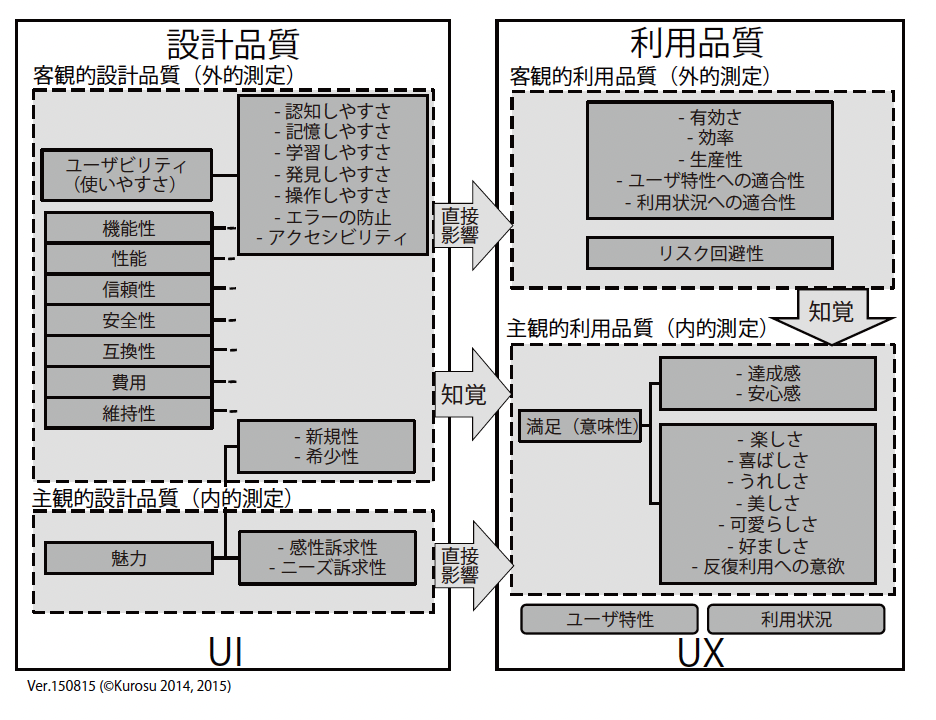
\includegraphics[width=100mm]{kurosu2015.png}}
    \end{center}
    \caption{黒須の品質特性図}
    \label{fig:kurosu2015}
  \end{minipage}
\end{figure}

\section{目的}



\section{本論文の構成}

本論文の構成を示す.

第\ref{chap:introduction}章では本研究の背景について述べた.第\ref{chap:prevresearch}章では関連研究と諸概念を整理する.第\ref{chap:pulsewave}章では脈波によるストレスチェックを応用したユーザビリティ評価手法を提案し,第\ref{chap:pulsewave}章ではそれを発展させた時系列ユーザビリティ評価手法を提案する.そして,それらの有効性を示す.最後に,第\ref{chap:conclusion}章の結論では本研究を総括し,考察と展望を述べる.付録として,本研究で行った実験で得られたデータを添付する.
